 \documentclass[]{article} 

\usepackage{xcolor}
\usepackage{tangocolors}

\definecolor{ljk}{rgb}{0.50, 0.625, 0.70}		

  \usepackage{tikz}

  \usetikzlibrary{calc,arrows,patterns,plotmarks,shapes,shapes.arrows,snakes,er,3d,automata,backgrounds,topaths,trees,petri,mindmap}

\begin{document}
\pagestyle{empty}
%\begin{frame}
\begin{center}

\tikzstyle{root concept}+=[concept color=white!80]
\tikzstyle{level 1 concept}+=[concept color=ljk!80, sibling angle=90]
\tikzstyle{every annotation}=[fill=black!50,opacity=0.5,text=black]
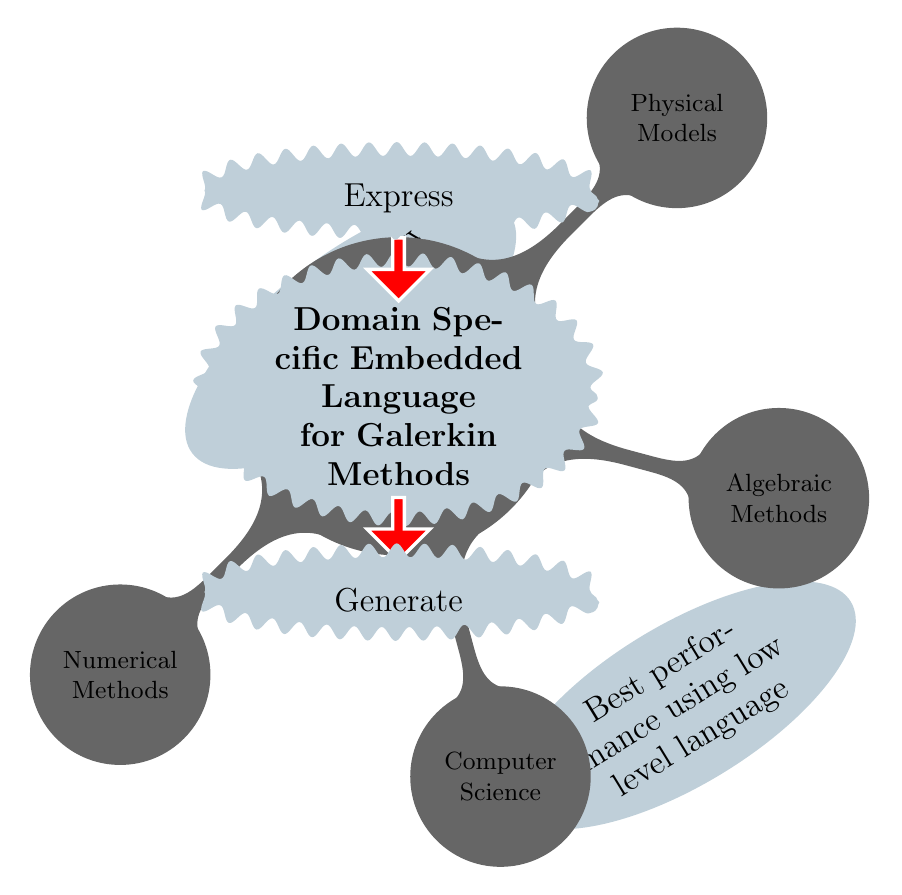
\begin{tikzpicture}[mindmap,concept color=black!60,text=black]
  %%\path[clip] (-6,0) rectangle (6,6);
  \node[concept,text=white] (root)  {Complexity of Scientific Computing Software}
  [clockwise from=45]
  child[concept] { node[concept] (mod) {Physical Models} }
  child[concept] { node[concept] (alg) {Algebraic Methods} }
  child[concept] { node[concept] (cs) {Computer Science} }
  child[concept] { node[concept] (num) {Numerical Methods} };
  
  \node[name=dsl,fill=ljk!50,ellipse,decorate,decoration=snake,minimum width=3cm,
  minimum height=2cm] at (root.center) {\bf Domain Specific
  Embedded Language for Galerkin Methods};
  
  \node[name=a1,single arrow, draw=white!80, rotate=-90,scale=.2,fill=red] at
  (dsl.north) {};
  \node[name=a2,single arrow, draw, white!80, rotate=-90,scale=.2,fill=red] at
  (dsl.south) {};
  \node[decorate,decoration=snake,fill=ljk!50,above,ellipse,minimum
  height=1cm] at (a1.west)  {Express};
  \node[decorate,decoration=snake,fill=ljk!50,below,ellipse,minimum height=1cm] at (a2.tip)  {Generate};
%  \node[single arrow, draw, gray!50, rotate=-45,scale=.2,fill=black!60] at
%  (dsl.south east) {Generate};


  \begin{pgfonlayer}{background}

    %\draw[pink,thick] (root.north east) -- (root.north west);

    \draw [concept connection,white] (num.west) --
    node[fill=ljk!50,above,sloped,text=black,ellipse,minimum height=1cm] {Best
    expressivity using high level language}
    (mod.east) ;

    \draw [concept connection,white]
    (cs.west) -- node[fill=ljk!50,below,sloped,text=black,ellipse,minimum
    height=1cm] {Best performance using low level language} (alg.east) ;

    %\draw[concept connection,-,white] (root.north west) -- (root.north east);

  \end{pgfonlayer} 



  % \path[fill=ljk!20,-] 
  % (root.north west)  .. controls (0,1cm) .. (root.north east) -- (root.south east) .. controls (0,-1cm) .. (root.south west) --  (root.north west);
\end{tikzpicture}
  
\end{center}
\end{document}
\vfill
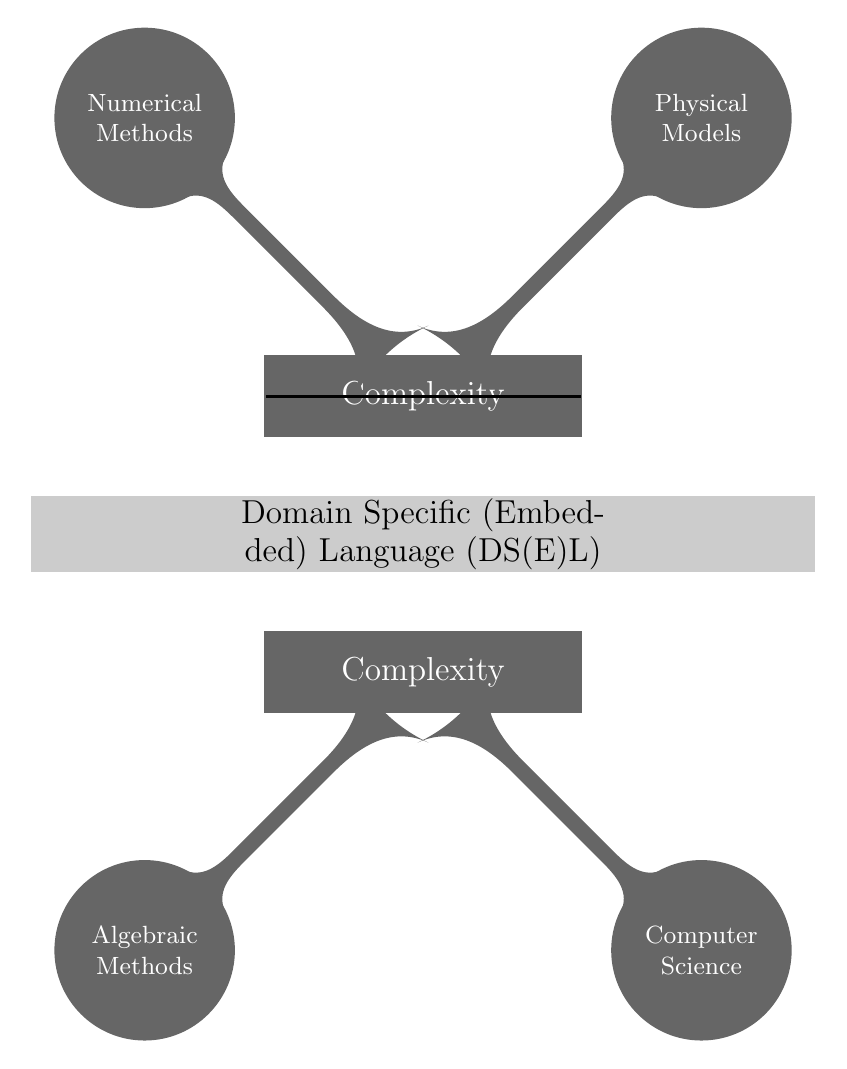
\begin{tikzpicture}[mindmap,concept color=black!60,text=white]
  \node[concept,rectangle,minimum height=1cm] (a) { Complexity}
  child[concept,grow=45] { node[concept] (mod) {Physical Models} }
  child[concept,grow=135] { node[concept] (num) {Numerical Methods} };
  

  \node[concept,below=3cm,rectangle,minimum height=1cm] (b) { Complexity}
  child[concept,grow=-45] { node[concept] (cs) {Computer Science} }
  child[concept,grow=225] { node[concept] (alg) {Algebraic Methods} };

  % \coordinate (A) at (a.center);
  % \coordinate (B) at (b.center);
  % \coordinate (C) at ($ (A!.5!B) $)

  \node[draw=white,fill=black!20,text=black,minimum width=10cm,minimum
  height=1cm,text width=7cm] at ($ (a.center)!.5!(b.center) $) {Domain Specific (Embedded)
  Language (DS(E)L)};
  \draw (a.east) -- (a.west);

\end{tikzpicture}
  
%\end{frame}

\end{document}
